\section{Introduction}

\begin{frame}{The farmer's problem {\small \cite{birge2011introduction}}}
	
	A farmer has available \alert{500 acres} of land available for raising wheat, corn, and sugar beets. 
	\begin{itemize}
		\item She needs at least \alert{200 tons of wheat} and \alert{240 tons of corn} for cattle feed;
		\item Cattle feed amounts can be \alert{raised} on the farm or \alert{bought} from a wholesale market;
		\item Sugar beet is raised for profit only. However, production above a \alert{6000 ton quota} has a lower sales price. 
	\end{itemize}	
	\pause
	\vspace{-6pt}
	{\small
	\begin{table}
		\begin{tabular}{r|ccc}
			& \bf Wheat & \bf Corn & \bf Sugar beets \\ \hline
			\bf Yield (ton/acre) & 2.5 & 3 & 20 \\
			\bf Planting cost (\$/acre) & 150 & 230 & 260 \\
			\bf Selling price (\$/ton) & 170 & 150  & 36 (under 6000 ton) \\
								   & 	 &	    & 10 (above 6000 ton) \\
			\bf Purchase price (\$/ton)& 238 & 210  & - \\ \hline					    
		\end{tabular}
		\caption{Farmer's problem data}		
	\end{table}
	}
	
\end{frame}


\begin{frame}{The farmer's problem {\small \cite{birge2011introduction}}}
	
	Let $I=\braces{1:\text{wheat}, 2:\text{corn}, 3:\text{sugar beets}}$. Then
	\vspace{-3pt}
	\begin{itemize}
		\item $x_i$	- acres devoted to $i$;
		\item $y_i$ - tons of $i$ purchased, $i \in I \setminus \braces{3}$;
		\item $w_i$ - tons of $i$ sold, $i \in I \cup \braces{4}$, $\braces{4: \text{sugar beets (over quota)}}$.
	\end{itemize}
	
	\pause
	The farmer's problem is:
	%
	\begin{align*}
		\mini & 150x_1 + 230 x_2 + 260 x_3 + 238 y_1 + 210 y_2 \\ & - 170 w_1 - 150 w_2 - 36 w_3 - 10w_4 \\
		\st & x_1 + x_2 + x_3 \le 500 \\
		& 2.5x_1 + y_1 - w_1 \ge 200 \\
		& 3 x_2 + y_2 - w_2 \ge 240 \\
		& w_3 + w_4 \le 20x_3 \\
		& w_3 \le 6000 \\
		& x_i \ge 0, i \in I; y_i \ge 0, i \in I \setminus \braces{3}; w_i \ge 0, i \in I \cup \braces{4}.
	\end{align*}
	%
\end{frame}


\begin{frame}{The farmer's problem {\small \cite{birge2011introduction}}}
	
	The optimal solution is given by:
	\vspace{6pt}
	\begin{columns}
	\column{0.35\textwidth}
		{\bf Optimal strategy}: 
		\begin{enumerate}
			\item plant sugar beets to \alert{reach} quota,
			\item satisfy \alert{minimum} requirements
			\item if in excess, sell the \alert{excess} as wheat; if in \alert{shortage}, purchase corn.
		\end{enumerate}	
	\column{0.60\textwidth}	
	\small
	\begin{table}
		\begin{tabular}{rccc}
					 & \bf Wheat & \bf Corn & \bf Sugar beets \\ \hline
			\bf Surface	 & 120	 & 80   & 300    	  \\
			\bf Yield	 & 300   & 240  & 6000     \\
			\bf Sales    & 100   & -    & 6000     \\  
			\bf Purchase & -     & -    & -        \\ \hline
			\multicolumn{3}{l}{\bf Overall profit:} & \$118,600  \\ \hline 
		\end{tabular}
		\caption{Optimal solution: average yields}
	\end{table}
	\end{columns}
	\pause
	\begin{itemize}
		\item The farmer is well aware that climate factors influence crop yields, which can \alert{fluctuate} $\pm$ 20\%.	
		\item How can we take these \alert{scenarios} into account for making land allocation decisions?
	\end{itemize}
	
\end{frame}


\begin{frame}{The farmer's problem {\small \cite{birge2011introduction}}}
	
	Considering the scenarios individually, we obtain:
	\vspace{-6pt}
	{\small
	\begin{table}
		\begin{tabular}{rccc}
					 & \bf Wheat  & \bf Corn & \bf Sugar beets \\ \hline
			\bf Surface	 & 183.33 & 66.67 & 250    	  \\
			\bf Yield	 & 550    & 240   & 6000     \\
			\bf Sales    & 350    & -     & 6000     \\  
			\bf Purchase & -      & -     & -        \\ \hline
			\multicolumn{3}{l}{\bf Overall profit:} & \$167,667  \\ \hline 
		\end{tabular}
		\caption{Optimal solution: \alert{20\% higher yields}}
	\end{table}
	\vspace{-9pt}
	\pause
	\begin{table}
		\begin{tabular}{rccc}
					 & \bf Wheat & \bf Corn & \bf Sugar beets \\ \hline
			\bf Surface	 & 100    & 25    & 375    	  \\
			\bf Yield	 & 200    & 60    & 6000     \\
			\bf Sales    & -      & -     & 6000     \\  
			\bf Purchase & -      & 180   & -        \\ \hline
			\multicolumn{3}{l}{\bf Overall profit:} & \$59,950  \\ \hline 
		\end{tabular}
		\caption{Optimal solution: \alert{20\% lower yields}}
	\end{table}
	}

\end{frame}


\begin{frame}{The farmer's problem {\small \cite{birge2011introduction}}}

	As one may notice, the land allocation for sugar beets is the \alert{critical} factor:
	
	\begin{itemize}
		\item Planting too much $\Rightarrow$ losses for selling above quota
		\item Planting too little $\Rightarrow$ opportunity losses
	\end{itemize}
	
	\pause
	We can \alert{hedge} against this uncertainty by taking a \alert{long-term perspective}:
	
	\begin{itemize}
		\item We assume that each year one of these scenarios happens. 
		\item We know they are \alert{equally likely} to happen, but exactly which will happen cannot be known.
		\item Thus, maximise \alert{long-run} profit $\Rightarrow$ maximise \alert{expected profit}.
	\end{itemize}
	
\end{frame}


\begin{frame}{The farmer's problem {\small \cite{birge2011introduction}}}
	
	Let $S = \braces{1: \text{-20\%}, 2: \text{avg.}, 3:\text{+20\%}}$ represent the \alert{yield scenarios}. 
	
	The reformulated farmer's problem is:
	%
	{\footnotesize
	\begin{align*}
		\mini & 150x_1 + 230 x_2 + 260 x_3 +~ \\
		& \frac{1}{3} (238 y_{11} + 210 y_{21} - 170 w_{11} - 150 w_{21} - 36 w_{31} - 10w_{41})\\
		& \frac{1}{3} (238 y_{12} + 210 y_{22} - 170 w_{12} - 150 w_{22} - 36 w_{32} - 10w_{42})\\
		& \frac{1}{3} (238 y_{13} + 210 y_{23} - 170 w_{13} - 150 w_{23} - 36 w_{33} - 10w_{43})\\
		\text{s.t.:~} & x_1 + x_2 + x_3 \le 500 \\
		&2x_1 + y_{11} - w_{11} \ge 200, \ 2.5x_1 + y_{12} - w_{12} \ge 200, \ 3x_1 + y_{13} - w_{13} \ge 200 \\
		& 2.4 x_2 + y_{21} - w_{21} \ge 240, \ 3 x_2 + y_{22} - w_{22} \ge 240, \ 3.6 x_2 + y_{23} - w_{23} \ge 240 \\
		& w_{31} + w_{41} \le 16x_3, \ w_{32} + w_{42} \le 20x_3, \ w_{33} + w_{43} \le 24x_3 \\
		& w_{31} \le 6000, w_{32} \le 6000, w_{33} \le 6000 \\
		& x_i \ge 0, i \in I; y_{is} \ge 0, i \in I \setminus \braces{3}, s \in S; w_{is} \ge 0, i \in I \cup \braces{4}, s \in S.
	\end{align*}
	}
	%
\end{frame}


\begin{frame}{The farmer's problem {\small \cite{birge2011introduction}}}

	The optimal solution becomes:
	
	{\small 
	\begin{table}
		\begin{tabular}{lrccc}
		   		 &	        & \bf Wheat & \bf Corn & \bf Sugar beets \\ \hline
		   		 & \bf Surface  & 170	& 80   & 250     	 \\ \hline
		   $s=1$ & \bf Yield	& 340   & 192  & 4000     \\
			   	 & \bf Sales    & 140   & -    & 4000     \\  
			     & \bf Purchase & -     & 48    & -        \\ \hline
		   $s=2$ & \bf Yield	& 422   & 240  & 5000     \\
			   	 & \bf Sales    & 225   & -    & 5000     \\  
			     & \bf Purchase & -     & -    & -        \\ \hline
		   $s=3$ & \bf Yield	& 510   & 288  & 6000     \\
			   	 & \bf Sales    & 310   & 48   & 6000     \\  
			     & \bf Purchase & -     & -    & -        \\ \hline
			\multicolumn{4}{l}{\bf Overall profit:} & \$108,390  \\ \hline 
		\end{tabular}
		\caption{Optimal solution: all scenario yields}
	\end{table}
	}
	
\end{frame}


\begin{frame}{The farmer's problem {\small \cite{birge2011introduction}}}

	By doing so, the farmer takes into account \alert{all scenarios simultaneously}.
	\vspace{-6pt}
	\begin{enumerate}
		\item The farmer exploits the \alert{timing} between making decisions and observing uncertainties;
		\item This ``hedging'' comes with a ``price'' that can be \alert{estimated} against perfect information performance.	
	\end{enumerate}
	
	\pause
	Effectively, this is achieved by incorporating \alert{decision stages} into the model:
	
	\begin{figure}
		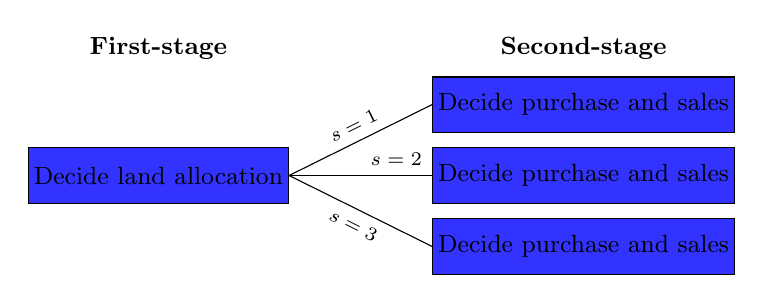
\begin{tikzpicture}[decision/.style={fill=blue!80, draw, minimum size=2em, inner 	sep=2pt}, scale=0.9, font=\small]
%			\draw[help lines] (0,0) grid (8,3);
			\node[decision] (1st-stage) at (1, 2) {Decide land allocation};
			\node[decision] (s1) at (7, 3) {Decide purchase and sales};
			\node[decision] (s2) at (7, 2) {Decide purchase and sales};
			\node[decision] (s3) at (7, 1) {Decide purchase and sales};
			\draw (1st-stage.east) edge node [sloped, above] {\scriptsize $s=1$} (s1.west);
			\draw (1st-stage.east) edge node [sloped, near end, above] {\scriptsize $s=2$} (s2.west);
			\draw (1st-stage.east) edge node [sloped, below] {\scriptsize $s=3$} (s3.west);
			\node (1st-stage label) at (1, 3.8) {\bf First-stage};
			\node (1st-stage label) at (7,3.8) {\bf Second-stage};
		\end{tikzpicture}	
	\end{figure}
	
\end{frame}


\begin{frame}{Two-stage stochastic programming}

	More formally, let:
	\vspace{-6pt}
	\begin{itemize}
		\item $x$ - definite (first-stage) decisions; 
		\item $y$ - corrective or recourse (second-stage) decisions;
		\item $\xi$ - \alert{random} variable;
		\item $[q(\xi), T(\xi), W(\xi), h(\xi)]$ - random vector (data);  	
	\end{itemize}
	
	\pause
	The formulation of a \alert{two-stage stochastic programming (2SSP)} model is
	%
	\begin{subequations} \label{eq:2SSP}
		\begin{align}
			\mini & c^\top x + \mathcal{Q}(x) \\
			\st  & Ax = b \\
			     & x \ge 0, 
		\end{align}
	\end{subequations}
	%
	where $\mathcal{Q}(x) = \mathbb{E}_\xi\brackets{Q(x, \xi)}$ and
	\begin{equation} \label{eq:2stage}
		Q(x, \xi) = \braces{\mini q(\xi)^\top y : W(\xi)y = h(\xi) - T(\xi)x, y \ge 0}.
	\end{equation}

\end{frame}


\section{Two-stage stochastic programming}


\begin{frame}{Two-stage stochastic programming}

	In essence, we are assuming the following \alert{decision process}
	$$
	 x \rightarrow \xi \rightarrow y(\xi, x)
	$$	
	in which $y$ is chosen to minimise $\mathbb{E}_\xi\brackets{Q(x, \xi)}$, assuming a \alert{known probability distribution} for $\xi$ with support $\Xi$.
	
	\pause
	Thus, we can pose problem \eqref{eq:2SSP} as the \alert{semi-infinite} problem
	%
	\begin{subequations} \label{eq:2SSP_2}
	\begin{align}
		\mini  & c^\top x + \mathbb{E}_\xi\brackets{Q(x, \xi)} \\
		\st	   & Ax = b, x \ge 0 \\
			   & T(\xi)x + W(\xi)y(\xi) = h(\xi), \ \forall \xi \in \Xi \\
			   & y(\xi) \ge 0, \ \forall \xi \in \Xi.
	\end{align}
	\end{subequations}

\end{frame}


\begin{frame}{Two-stage stochastic programming}
	
	There are two complicating factors in \eqref{eq:2SSP_2}:
		\vspace{-6pt}
	\begin{enumerate}
		\item $\mathbb{E}_\xi\brackets{Q(x, \xi)}$; 
		\item $\forall \xi \in \Xi$.	
	\end{enumerate}
	
	\pause
	Those are treated by means of \alert{discretisation}, that is: 
	\vspace{-6pt} 
	\begin{itemize}
		\item In general, we assume $\Xi$ to be a \alert{discrete} and \alert{finite} set;
		\item Each realisations $\xi_s \in \Xi$, for $s \in S \equiv \braces{1, \dots, |\Xi|}$ is a \alert{scenario};
		\item Thus,	$[q(\xi), T(\xi), W(\xi), h(\xi)]$ becomes a discrete and finite set of parameters:
		\begin{align*}
			 [&q(\xi_1), T(\xi_1), W(\xi_1), h(\xi_1); \\
			    &q(\xi_2), T(\xi_2), W(\xi_2), h(\xi_2); \\
			    &\dots ;\\
				& q(\xi_{|\Xi|}), T(\xi_{|\Xi|}), W(\xi_{|\Xi|}), h(\xi_{|\Xi|})] \\
				\Rightarrow~ & [q_s, T_s, W_s, h_s] = \xi_s, s \in S.
		\end{align*}
	\end{itemize}
	
\end{frame}


\begin{frame}{Two-stage stochastic programming}

	Considering a finite and discrete set of scenarios, we can restate \eqref{eq:2SSP_2} as its \alert{deterministic equivalent}
	%
	\begin{subequations} \label{eq:2SSP_DE}
	\begin{align}
		\mini  & c^\top x + \sum_{s\in S} P_s q_s^\top y_s \\
		\st	   & Ax = b, x \ge 0 \\
			   & T_sx + W_s y_s = h_s, \ \forall s \in S \\
			   & y_s \ge 0, \ \forall s \in S.
	\end{align}
	\end{subequations}
	\pause 
	{\bf Remark:} notice how discretisation solves the tractability issues:
	\vspace{-6pt}
	\begin{enumerate}
		\item $P_s$ is the probability associated with scenario $s$ ($P_s = P(\xi = \xi_s)$). Thus $\mathbb{E}_\xi\brackets{Q(x, \xi)} = \sum_{s\in S} P_s q_s^\top y_s$.
		\item \eqref{eq:2SSP_DE} has a \alert{finite} number of variables and constraints.	
	\end{enumerate}


	
\end{frame}


\begin{frame}{Two-stage stochastic programming}
	
	In the farmer's problem, there we assumed that $s \in \braces{1,2,3}$:
		\vspace{-6pt}
		\begin{itemize}
			\item $q_s = q_{s'}$, $W_s = W_{s'}$, and $h_s = h_{s'}$, $\forall s, s' \in S \mid s \neq s'$;
			\item $T_s = \brackets{t_1(s), t_2(s)}$.  	
		\end{itemize}
	
	\pause
	And thus, we had that:
	\begin{align*}
		Q_s(x) = \mini \ &238y_1(s) -170w_1(s) + 210y_2(s) - 150w_2(s) \\
		& \quad -36w_3(s) -10w_4(s) \\
		\st   \ & \alert{t_1(s)}x_1 + y_1(s) - w_1(s) \geq 200 \\
                & \alert{t_2(s)}x_2 + y_2(s) - w_2(s) \geq 240 \\
                & w_3(s) + w_4(s) \leq t_3(s)x_3 \\
                & w_3(s) \leq 6000 \\
                & y_1(s), w_1(s), y_2(s), w_2(s), w_3(s), w_4(s) \geq 0. 
	\end{align*}

	
\end{frame}


\section{Measures of quality: EVPI and VSS}


\begin{frame}{The expected value of perfect information (EVPI)}

	The performance of the solution of a 2SSP can be compared against a so-called \alert{wait-and-see} (WS) solution.
	
	Let our 2SSP be compactly represented as
	\begin{equation*}
		z = \mini_x \braces{\mathbb{E}\brackets{F(x,\xi)}}, 	
	\end{equation*}
	where $F(x,\xi) = \braces{c^\top x + \mathbb{E}\brackets{Q(x,\xi)} : x \in X}$, $Q(x,\xi)$ is defined as \eqref{eq:2stage}, and $X=\braces{x \in \reals^n : Ax = b, x \ge 0}$.
	
	\pause
	A WS solution can be obtained from a \alert{perfect-foresight} version
	\begin{equation*}
		z^{\text{WS}} = \mathbb{E}_\xi\brackets{\mini_x \braces{F(x,\xi)}} = \mathbb{E}_\xi\brackets{F(x(\xi), \xi)},
	\end{equation*}
	%
	where $x(\xi) = \argmin_x \braces{F(x,\xi)}$.
	
	\pause
	Then, the expected value of perfect information (EVPI) is: 
	$$
		EVPI = z - z^{\text{WS}}.
	$$
\end{frame}


\begin{frame}{Value of stochastic solution (VSS)}

	We can also compare the solution of a 2SSP against a \alert{reference (first-stage) solution}. 
	
	For that, let $\overline{\xi}$ be a reference scenario (realisation). Then
	$$
		x(\overline{\xi}) = \argmin_x F(x, \overline{\xi}) 
	$$
	represents the optimal solution associated with that scenario.
	
	\pause
	
	We can then calculate the performance of $x(\overline{\xi})$ against $\xi \in \Xi$:		 
	$$
		z^{\text{EV}} = \mathbb{E}_\xi\brackets{F(x(\overline{\xi}), \xi)}.
	$$
	If $\overline{\xi} = \mathbb{E}\brackets{\xi}$, we have the \alert{value of the stochastic solution (VSS)}:
	$$
		VSS = z^{\text{EV}} - z.
	$$
	
\end{frame}

	
\begin{frame}{EVPI and VSS - general remarks}

	Some relevant observations:
	\vspace{-6pt}
	\begin{itemize}
		\item With minimisation as a reference, we have that
		$$
			z^{\text{WS}} \le z \le z^{\text{EV}} \Rightarrow EVPI \ge 0, VSS \ge 0.
		$$
		\item Stronger statements are possible if assumptions on the 2SSP problem structure or the uncertainty terms are made.
		\item VSS: the \alert{higher} the better;
		\item EVPI: the \alert{lower} the better.
	\end{itemize}
	
	\pause
	For the farmer's example:
	\vspace{-6pt}
	\begin{itemize}
		\item $EVPI = -108,390- \left(\frac{1}{3}\times -167,777 + \frac{1}{3}\times -118,000 + \frac{1}{3}\times -59,950\right)  = \$7016$ 
		\item $z^{\text{EV}} = -107,240$\footnote{Calculated by fixing the solution $x=(120,80,300)$ for each scenario and taking the average of the objective function values}; $VSS = -107,240 - (-108,390) = \$1150$
	\end{itemize}
	\vspace{6pt}
\end{frame}


\section{Recourse types}


\begin{frame}{Types of recourse problems}

	It is common to classify 2SSP according to their \alert{recourse problem} 
	\begin{equation*}
		Q(x, \xi) = \braces{\mini q(\xi)^\top y : W(\xi)y = h(\xi) - T(\xi)x, \ y \ge 0}.	
	\end{equation*}
	
	Most common structures:
	\begin{enumerate}[<+->]
		\item {\bf Fixed recourse:} means that $W(\xi) = W$, $\forall \xi \in \Xi$.
		\item {\bf Simple recourse:} In that case, $W = I$, reducing the recourse feasibility condition to $y = h(\xi) - T(\xi)x$. 
		\vspace{6pt}
		
		This implies that the recourse becomes
		$$
		 Q(x,\xi) = h(\xi) - T(\xi)x.
		$$ 
	\end{enumerate} 
	
\end{frame}


\begin{frame}{Types of recourse problems}
	
	\begin{enumerate}[<+->]
		\item[3.] {\bf Complete recourse:} relates to the \alert{feasibility} of the recourse problem. If the 2SSP has complete recourse, then
		\begin{align*}
			& Q(x,\xi) < \infty, \ \forall \xi \in \Xi \Longleftrightarrow \\
			& \braces{y : W(\xi)y = h(\xi) - T(\xi)x, y \ge 0} \neq \emptyset, \ \forall \xi \in \Xi 
		\end{align*}
	    \item[4.] {\bf Relatively complete recourse:} in this case, the feasibility of the recourse problem is \alert{conditioned} on $x \in X$
		\begin{align*}
			& Q(x,\xi) < \infty, \ \forall \xi \in \Xi, x \in X \Longleftrightarrow \\
			& \braces{y : W(\xi)y = h(\xi) - T(\xi)x, y \ge 0} \neq \emptyset, \ \forall \xi \in \Xi, x \in X. 
		\end{align*}
	\end{enumerate}

	
\end{frame}


\section{Multi-stage problems}


\begin{frame}{Beyond two decision stages} 

	Many problems have in fact multiple decision points, in which decisions are made  \alert{sequentially}.
	\vspace{-12pt}
	%
	\begin{figure}
		\centering
		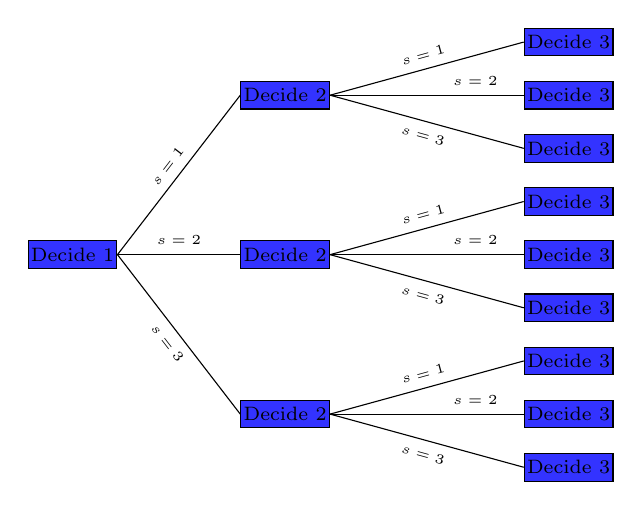
\begin{tikzpicture}[decision/.style={fill=blue!80, draw, minimum size=1em, inner sep=1pt, font=\scriptsize}, font=\tiny, scale = 0.9]
%			\draw[help lines] (0,0) grid (8,3);
			\node[decision] (1st-stage) at (1, 2) {Decide 1};
			\node[decision] (s1) at (4, 4.25) {Decide 2};
			\node[decision] (s2) at (4, 2) {Decide 2};
			\node[decision] (s3) at (4, -0.25) {Decide 2};
			\node[decision] (s11) at (8, 5) {Decide 3};
			\node[decision] (s12) at (8, 4.25) {Decide 3};
			\node[decision] (s13) at (8, 3.5) {Decide 3};
			\node[decision] (s21) at (8, 2.75) {Decide 3};
			\node[decision] (s22) at (8, 2) {Decide 3};
			\node[decision] (s23) at (8, 1.25) {Decide 3};
			\node[decision] (s31) at (8, 0.5) {Decide 3};
			\node[decision] (s32) at (8, -0.25) {Decide 3};
			\node[decision] (s33) at (8, -1) {Decide 3};
			\draw (1st-stage.east) edge node [sloped, above] {$s=1$} (s1.west);
			\draw (1st-stage.east) edge node [sloped, above] {$s=2$} (s2.west);
			\draw (1st-stage.east) edge node [sloped, below] {$s=3$} (s3.west);
			\draw (s1.east) edge node [sloped, above] {$s=1$} (s11.west);
			\draw (s1.east) edge node [sloped, near end, above] {$s=2$} (s12.west);
			\draw (s1.east) edge node [sloped, below] {$s=3$} (s13.west);
			\draw (s2.east) edge node [sloped, above] {$s=1$} (s21.west);
			\draw (s2.east) edge node [sloped, near end, above] {$s=2$} (s22.west);
			\draw (s2.east) edge node [sloped, below] {$s=3$} (s23.west);
			\draw (s3.east) edge node [sloped, above] {$s=1$} (s31.west);
			\draw (s3.east) edge node [sloped, near end, above] {$s=2$} (s32.west);
			\draw (s3.east) edge node [sloped, below] {$s=3$} (s33.west);
		\end{tikzpicture}	
	\end{figure}
	
\end{frame}



\begin{frame}{Beyond two decision stages} 

	\alert{Multi-stage} decision problems:
	\vspace{-6pt}
	\begin{enumerate}
		\item Consist of \alert{nested two-stage problems}. This can be exploited in a \alert{dynamic programming} fashion;
		\item Likewise, presents \alert{exponential growth} with scenarios per stage ($|\Xi|^{|H|-1}$, with $|\Xi|$-scenario stages $t \in [H]$%
		%
		\footnote{$n \in [N] = n \in \braces{1,\dots,N}.$}
		%
		);
		\item Trade-off: future \alert{flexibility} versus computational cost.	
	\end{enumerate}
	
	\pause
	Consider that we have $H$ decision stages. Our decision process becomes:
	%
	\begin{align*}
		& x^1 \rightarrow \xi^2 \rightarrow x^2(\xi^2,x^1)
	 	 \rightarrow \xi^3
	 	 \rightarrow x^3((\xi^2,\xi^3), (x^1,x^2)) \rightarrow \dots \\\rightarrow 	
	 	 ~& \xi^H \rightarrow x^H((\xi^2,\dots,\xi^H), (x^1,\dots,x^{H-1}))
	\end{align*}
	
	\vspace{-6pt}	
	\begin{itemize}
		\item $\xi$ up to stage $t= 2, \dots, T$ represents a \alert{sequence} of events
		\item Hereinafter, $x^t(\xi)$ is a shorthand for $x^t((\xi^2,\dots,\xi^t))$ \vspace{6pt}	
	\end{itemize}
	 

\end{frame}

\begin{frame}{Multi-stage decision problems} 

	For $t = H$ we have:
	%
	\begin{align*}
		 Q^H(x^{H-1},\xi^H) = \mini & c^H(\xi)^\top x^H(\xi) \\
		 \st & W^H(\xi) x^H(\xi) = h^H(\xi) - T^{H-1}(\xi)x^{H-1} \\
		 &x^H(\xi) \ge 0.  
	\end{align*}
	
	\pause
	For $t = 2, \dots, H-1$ we have:
	%
	\begin{align*}
		 Q^t(x^{t-1},\xi^t) = \mini & c^t(\xi)^\top x^t(\xi) + \mathcal{Q}^{t+1}(x^t)\\
		 \st & W^t(\xi) x^t(\xi) = h^t(\xi) - T^{t-1}(\xi)x^{t-1} \\
		 &x^t(\xi) \ge 0.  
	\end{align*}
	\vspace{-6pt}
	\pause
	We want to solve
	%
	\begin{align*}
		  \mini & c^{1\top} x^1 + \mathcal{Q}(x^1) \\
		 \st & W^1x^1 = h^1 \\
		 &x^1 \ge 0.  
	\end{align*}
	

\end{frame}


\begin{frame}{Example: 3SSP}

A \alert{3-stage} formulation is given as:
	%
	\begin{flalign*}
	\mini & c^{1\top}  x^1 + \sum_{\xi^2_s \in S^2}P(\xi^2_s)\left[c^2(\xi^2_s)^\top x^2(\xi^2_s) + \right. \\ &  \sum_{\xi^3_s \in S^3(\xi^2_s)}\left. P(\xi^3_s | \xi^2_s)\left({c^3(\xi^3_s | \xi^2_s)}^\top x^3(\xi^3_s | \xi^2_s) \right)\right] \\
	\st & T^1 x^1 = h^1 \\
		& T(\xi^2_s)x^1 + W(\xi^2_s)x^2(\xi^2_s) = h(\xi^2_s), \forall \xi^2_s \\
		& T(\xi^3_s | \xi^2_s) x^2(\xi^2_s) + W(\xi^3_s | \xi^2_s)x^3(\xi^3_s | \xi^2_s) = h(\xi^3_s | \xi^2_s), \forall \xi^2_s, \xi^3_s | \xi^2_s \\
		&x^1 \ge 0 \\
		&x^2(\xi^2_s) \ge 0, \ \forall \xi^2_s \\
		&x^3(\xi^3_s | \xi^2_s) \ge 0, \ \forall \xi^2_s, \xi^3_s|\xi^2_s.
	\end{flalign*}

\end{frame}


\begin{frame}{References}

	\bibliographystyle{apalike}
	\bibliography{../aux/references.bib}
	
\end{frame}
